\chapter{Implementierung}
Das Ziel der Projektarbeit ist sowohl ein Offline- als auch ein Online-Modus zu implementieren und insbesondere mit dem Offline-Modus die eingesetzten Algorithmen zu vergleichen. Im diesem Kapitel werden die Kernmodule, die für beide Modi benötigt werden, sowie die einzelnen Modi beschrieben. Des Weiteren wird im letzten Abschnitt ein Evolutionärer Algortihmus zur Parameteroptimierung beschrieben.

\section{Kernmodule}
Der Kern sämtlicher Implementierungen stellen verschiedene Module dar, die für verschiedene Einsatzzwecke benutzt werden können. Bei jedem Modul handelt es sich um ein ausführbares Programm. In Abbildung \ref{fig:moduluebersicht} sind alle Kernmodule dargestellt. Gelb markiert sind die eigens für das Projekt in Java implementierten Module, blau markiert sind Module, die aus der \emph{libsvm} (Version 3.12) stammen. Die Kernmodule decken die in Kapitel \ref{cha:theorie} beschrieben vier Arbeitsschritte vollständig ab. 

\begin{description}
	\item[Preprocessing] Im Modul \emph{FeatureExtraction} werden die einkommenden Wav-Dateien (Mono, 16 kHz, 16 Bit) in Featurevektoren umgewandelt. Die Umwandlung erfolgt über LPC oder MFCC, wobei für MFCC die Bibliothek \emph{CoMIRVA} verwendet wird. \cite{bib:comirva} Für die Verwendung von SVM in Trainings- und Prediction-Phase ist eine Skalierung von Vorteil. Hierzu wird das Modul \emph{SvmScale} der \emph{libsvm} verwendet.
	\item[Training] Das Training kann auf zweierlei Arten durchgeführt werden. Zum einen wird durch das Modul \emph{SvmTrain} der \emph{libsvm} ein SVM-Klassifikator zur Verfügung gestellt. Zum anderen wird durch \emph{CreateCodebook} ein Codebuch auf Basis des Neural Gas Algorithmus erzeugt.
	\item[Prediction] Wurde beim Training SVM verwendet, wird in dieser Phase das Modul \emph{SvmPrediction} der \emph{libsvm} verwendet. Wurde dagegen ein Codebuch erstellt, wird die Methode des nächsten Nachbarn mit dem Modul \emph{NearestNeighbor} verwendet.
	\item[Analysis] Das Modul \emph{Analysis} wertet die Ergebnisse der Prediction-Phase aus und speichert sowohl die Erkennungsrate, als auch eine Verwechslungsmatrix in einer Ausgabedatei.
\end{description}

Zum Informationsaustausch zwischen den Modulen wird das bestehende Dateiformat der \emph{libsvm} benutzt. Dadurch ist die Interoperabilität mit der \emph{libsvm} gewährleistet, ohne dass ein Wrapper dafür benötigt wird.

\begin{figure}[h]
  \centering
  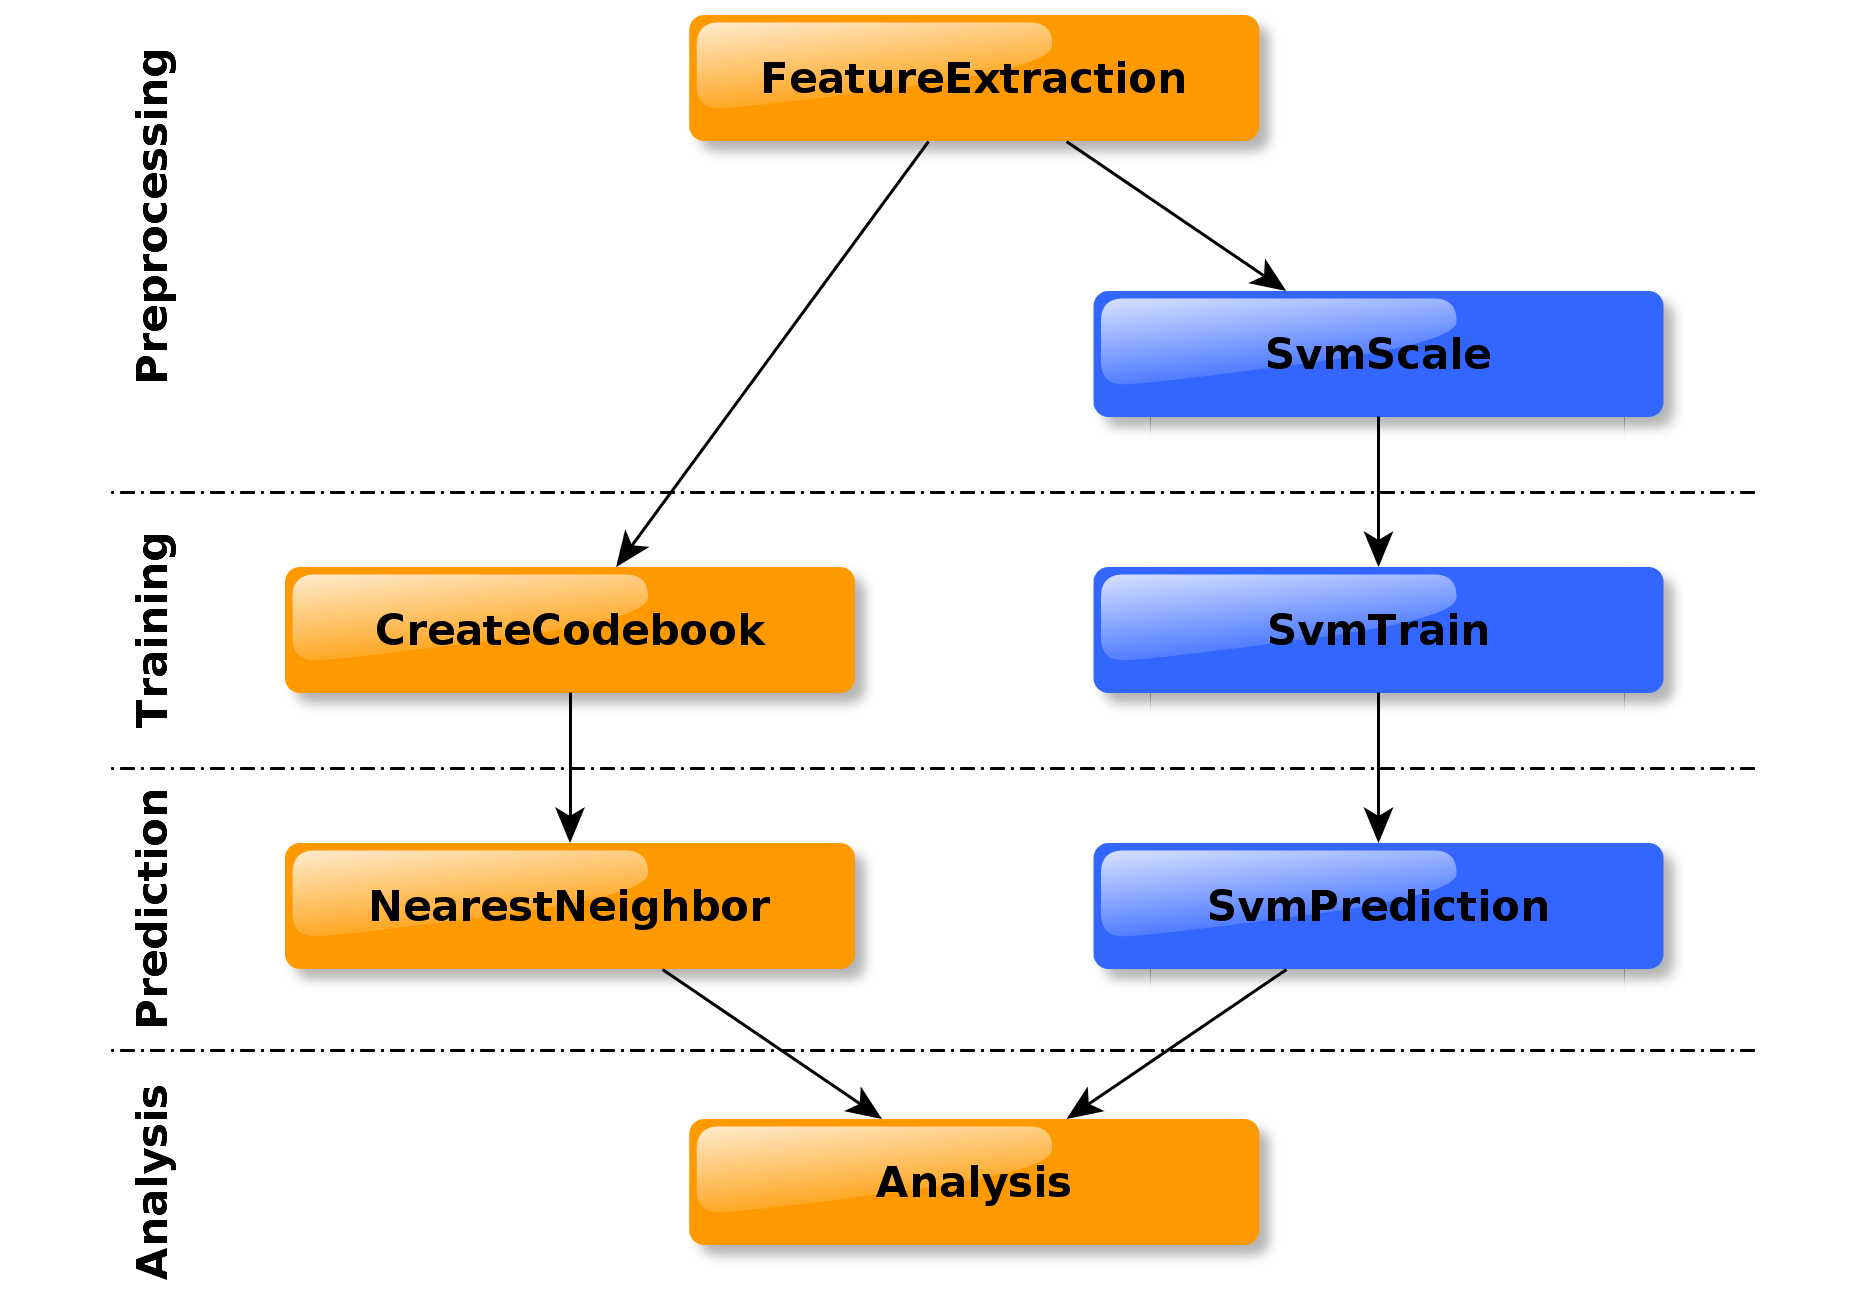
\includegraphics[width=1\textwidth]{images/moduluebersicht}
  \caption{Kernmodule in der Übersicht}
  \label{fig:moduluebersicht}
\end{figure}

Der Vorteil in der Modularisierung liegt in der flexiblen Anwendung. So kann beispielsweise unkompliziert getestet werden, ob die Skalierung auch beim Einsatz von \emph{Neural Gas} sinnvoll ist. Des Weiteren können die Module für weitere Einsatzzwecke genutzt werden. Um zum Beispiel eine Gesichts- oder Texterkennung zu implementieren müsste nur das \emph{FeatureExtraction}-Modul ausgetauscht werden. Der Nachteil einer solchen Modularisierung stellen die beschränkten Debuggingmöglichkeiten dar. Da es sich um für sich jeweils abgeschlossene Programme handelt, kann man nicht auf herkömmliche Weise im Programmcode debuggen.

\section{Offline-Test}
Ein Bash-Skript dient der Vergleichbarkeit der Ergebnisse. Dieses ermöglicht die Veränderung sämtlicher Einstellungen, wie die Fensterbreite der Featurevektoren oder der Trainingsmethode. Das Skript führt eine Kreuzvalidierung über drei Blöcke durch und speichert das Analyseergebnis in einer Datei.

\section{Online-Modus}
Ein Java-Programm stellt den Online-Modus der Sprechererkennung dar. Dieses verwendet MFCC in der Preprocessing-Phase und Neural Gas in der Trainingsphase. Diese Algorithmen werden verwendet, da sie zum Zeitpunkt der Implentation subjektiv am effizentisten arbeiteten. Das Programm ist so implementiert, dass es immer nach 320 ms ein Statusupdate auf der Konsole ausgibt. In diesem wird der Sprecher über die letzten 1,6 Sekunden ermittelt, wobei neuere Werte stärker gewichtet werden. Die einzelnen Gewinner der neuesten Feature-Vektoren werden 5-fach so stark gewichtet, wie die der ältesten Feature-Vektoren. Die Gewichtung nimmt linear mit dem Alter der Feature-Vektoren ab.

\section{Evolutionärer Algorithmus zur Parameteroptimierung}
Betrachtet man die einstellbaren Parameter für MFCC und Neural, ergibt dies einen 7-dimensionalen Vektorraum in dem das Optimum der Parameter gefunden werden soll. Die einzelnen Parameter sind:
\begin{itemize}
	\item Fensterbreite
	\item Überlappung der Fenster
	\item Merkmale pro Fenster
	\item Minmale Energielevel
	\item Fensterfunktion (Hamming oder Hann)
	\item Größe des Codebuchs
	\item Iterationen des Neural Gas Algorithmus
\end{itemize}
Sollte die Fensterbreite veränderbar sein, lassen sich die Ergebnisse nur noch schwer vergleichen, da mit der Fensterbreite auch die Information pro Fenster steigt. Somit wurde diese Einstellung auf 32 ms Fensterbreite fixiert.

Um das Optimum in dem noch verbleibenden 6-dimensionalen Vektorraum zu finden, dient ein Evolutionärer Algorithmus. Dabei wird eine variable Mutationsrate eingesetzt, da diese lokale Optimas besser vermeidet, als eine statitische Mutationsrate. Die Fitnessfunktion stellt die Funktion \ref{equ:fitness} dar. Als Eingabeparameter dienen der Funktion die für den Durchlauf mit den aktuellen Parametern benötigte Zeit in Sekunden $t$, sowie die Erkennungsrate auf Einzelfenster in Prozent $acc$. Zur Selektion dient eine Tournament-Selektion, bei de je vier Individuen gegen einander antreten, wobei nur der beste in die nächste Population gelangt. Eine Population besteht aus 12 Individuen. 

\begin{equation}
	\label{equ:fitness}
	\begin{aligned}[t]f(t,acc) = \frac{acc}{1 - e^{\left(\frac{-t}{1000}\right)}}\end{aligned}
\end{equation}
